\documentclass[11pt]{article}

% ACL style: "preprint" = non-anonymous with page numbers. Use "review" for an anonymous version, "final" for camera-ready.
\usepackage[preprint]{acl}

\usepackage{times}
\usepackage{latexsym}
\usepackage[T1]{fontenc}
\usepackage[utf8]{inputenc}
\usepackage{microtype}
\usepackage{inconsolata}
\usepackage{graphicx}
\usepackage{booktabs}
\usepackage{xcolor}
\usepackage{tikz}
\usetikzlibrary{shapes.geometric,positioning,fit,backgrounds,arrows.meta,calc}

% ---------------------------------------------------------------- draft mode
% \todo{...} marks a number or fact still to be filled. Visible in the PDF while \drafttrue.
% For a clean copy set \draftfalse (the todo text then disappears; check that no sentence is left empty).
\newif\ifdraft
\drafttrue
\newcommand{\todo}[1]{\ifdraft{\color{red}\textbf{[TODO: #1]}}\fi}

% ---------------------------------------------------------------- generated result tables
% Tables written by `python -m vakeel_sahayak.eval.scoring report` land in docs/results/dev-sweep/tables/.
% A missing file leaves a visible placeholder, so the document compiles with or without them.
\newcommand{\tabdir}{../results/dev-sweep/tables}
\newcommand{\resulttable}[2]{% #1 = file stem, #2 = "n" narrow (one column) or "w" wide (two columns)
  \IfFileExists{\tabdir/#1.tex}{%
    \begingroup
    \if#2w\let\table\table*\let\endtable\endtable*\let\small\scriptsize\fi
    \input{\tabdir/#1.tex}%
    \endgroup
  }{%
    \par\smallskip\noindent\fbox{\parbox{0.9\linewidth}{\footnotesize \ifdraft\color{red}\fi Table \texttt{\detokenize{#1}} not generated yet (scoring pipeline output).}}\par\smallskip
  }%
}

\newcommand{\resref}[1]{\IfFileExists{\tabdir/#1.tex}{Table~\ref{tab:#1}}{the table \texttt{\detokenize{#1}}}}

\title{Vakeel-Sahayak.ai: An Agentic Harness for Bail Preparation\\ over Typed Legal Stores (Status Report)}

\author{Vishak Kashyap K \and Shravani K \and Satvik Rao \and Harshita Kumari \\
  International Institute of Information Technology, Hyderabad \\
  \texttt{vishakkashyap.k@research.iiit.ac.in}}

\begin{document}
\maketitle

\begin{abstract}
Legal-aid lawyers in India prepare bail applications from messy case files: scanned and photographed orders, Hindi and English, several documents merged in one PDF. We describe Vakeel-Sahayak.ai, a bail-preparation engine built as an agent harness rather than a single model call. Six agents (intake, dossier and rights checks, retrieval orchestration, drafting, prosecution sparring, batch triage) work over ten typed stores on four shelves. An orchestrator reads a short evidence contract for each of twelve bail factors and decides which stores to query, in which order, and when to stop. Every claim in a draft is checked against its sources, and a draft changes only where a dependency changed. Two approval gates are enforced in code, and client text passes a pseudonymisation boundary before any external model sees it. We evaluate without manual annotation: gold labels come from court text, with a rule labeler and a non-Qwen model labeler that must agree and quote a verbatim span. We compare the full system with seven simpler baselines (single pass, single store, whole-document embeddings, naive chunking, query-every-store, a learned store router, and an expert rule list) and with 18 single-switch variants taken from recent agent and RAG papers. This report describes the system and the evaluation design, and states what has run so far. On the 50-case development set the full system reaches \todo{factor recall, Full vs.\ B0--B4, from \texttt{table1\_main}}, with an unsupported-fact rate of \todo{M6 from \texttt{table1\_main}} and a cost of \todo{USD per case from \texttt{table9\_cost}}. These numbers are preliminary: small $n$, development data only, and stand-in models in places.
\end{abstract}

\section{Introduction}

\paragraph{Problem.} A legal-aid lawyer who prepares a regular bail application in an Indian High Court (CrPC s.439, now BNSS s.483) starts from a pile of documents: a born-digital High Court order, a scanned Sessions Court order, a phone photo of an FIR copy, remand orders and a custody certificate, often merged into one PDF and often in Hindi. The application needs exact statute text, a mapping from old to new sections since the 2024 change from IPC and CrPC to BNS and BNSS, court reasoning on each bail factor, the citation history of every authority, and the case's own timeline. No single vector index serves all of these. A model asked to write it from memory fabricates facts and case law, as studies of commercial legal research tools found \citep{magesh2025}.

The problem is one of data engineering and decisions before it is one of text generation: the input is heterogeneous, the knowledge has several shapes, each factor needs evidence from different places, the case keeps moving, and an office has hundreds of files to triage.

\paragraph{Why agentic.} Three of these steps involve a decision that depends on what was just found: how far down a parse ladder a page must go, which store to ask next for a given factor and whether the result is enough, and which part of a draft a new order has made stale. A fixed pipeline either does too much (every store, the vision model on every page) or too little. We built the decisions as agents with typed tools, typed hand-offs and budgets, and we measure each of them against a simpler alternative.

\paragraph{Scope.} Users are panel lawyers, junior advocates and supervised legal-aid clinics. The system does not predict outcomes, show grant rates, or advise accused persons or the public.

\paragraph{Contributions.} The research contribution is the harness and its evaluation, not a new model.
\begin{enumerate}\setlength\itemsep{0pt}
\item \textbf{The harness.} Six court-office agents over ten typed stores on four shelves; page-level agentic ingestion for ten input kinds; an orchestrator that plans retrieval per factor (Section~\ref{sec:system}).
\item \textbf{Evidence contracts.} For each of twelve bail factors, a short declarative list of the evidence a ground needs and which stores may hold it. The contract fixes what is needed and where it may be; the orchestrator decides the order, the query, sufficiency and the stop.
\item \textbf{Truth maintenance for drafts.} Each claim stores its dependencies. When counsel approves a change, only stale claims are redrafted and all other claims stay byte-identical, an idea from classical truth-maintenance systems \citep{doyle1979tms}.
\item \textbf{Two gates in code.} Counsel approves the dossier (Gate~1) and the brief (Gate~2). Export is impossible before Gate~2, and approvals can only come from counsel.
\item \textbf{Evaluation without manual annotation.} Seven kinds of gold label and nine test sets built from court text, official tables and construction; a sealed blind slice and a pre-registration; baselines B0 to B6; 18 single-switch variants from the recent agent and RAG literature, each with a switch, a paper and a test (Section~\ref{sec:eval}).
\end{enumerate}

This is a status report. The system, the test sets and the scoring pipeline are built. The dev-set runs on the pinned code tag exist on disk but are not scored, and no further paid runs are planned for now, so Section~\ref{sec:results} is a template that is filled from generated tables.

\section{Related Work}

\paragraph{Agentic and adaptive RAG.} Self-RAG and CRAG let the model critique retrieved text and re-retrieve \citep{asai2024selfrag,yan2024crag}; Adaptive-RAG chooses the retrieval depth by query complexity \citep{jeong2024adaptive}; Sufficient Context studies when the retrieved context is enough to answer \citep{joren2025sufficient}; HippoRAG~2 retrieves over a graph \citep{gutierrez2025hipporag2}. We implement adaptations of these as opt-in switches (S1, S2, S3, S5) and compare them with hand-written contracts. A related line routes among language models or answering agents \citep{zhang2026agentrouter}; our action space is about ten stores that are not agents, so a learned store prior is only one baseline (B5) and one ablation (S6).

\paragraph{Multi-agent systems and verification.} Self-critique without an outside verifier is reported to help little \citep{gou2024critic,huang2024selfcorrect}; we keep an NLI and rule-based check as the critic and add a self-critique arm (S8) to test this in our domain. For adversarial review, debate gains are partly explained by voting \citep{choi2025debate}, and context sharing can hurt \citep{wynn2025talk}. These motivate our prosecution-sparring ablations (S9, S10). \citet{cemri2025mast} give a taxonomy of multi-agent failures. AgentCourt and CourtEval place agents in court roles \citep{chen2025agentcourt,kumar2025courtevel}; our opponent is scored against objections the real prosecution raised.

\paragraph{Ingestion and chunking.} VisRAG and ColPali retrieve over page images \citep{yu2025visrag,faysse2025colpali}; we use an image-only arm as a baseline for a text-first routing ladder. Dense X Retrieval studies the granularity of retrieval units \citep{chen2024densex}; our naive-chunking baseline B3 and the proposition-unit variant S16 test this on court orders.

\paragraph{Legal NLP.} Work on Indian courts is mostly judgment or outcome prediction \citep{nigam2025nyayarag,nigam2024predex}. \citet{magesh2025} show that commercial legal RAG tools still fabricate and misground citations. We cite them for positioning and design the metrics around that finding: every citation is looked up, and every quoted span must appear verbatim in the cited paragraph. Counter-argument retrieval as a separate kind of evidence \citep{wachsmuth2018} motivates our authority-stance variant (S18).

\paragraph{Evaluation.} For grounding we use MiniCheck \citep{tang2024minicheck} and an NLI model, and citation precision and recall in the style of ALCE \citep{gao2023alce}. No score in this report comes from an LLM judge.

\paragraph{Safety and serving.} Typed hand-offs follow design patterns for securing agents \citep{beurerkellner2025patterns}; batch scheduling follows serving work such as SGLang \citep{zheng2024sglang}. Both are opt-in arms (S17, S14).

\section{System}
\label{sec:system}

Figure~\ref{fig:arch} shows the system. The agents are named after people in an Indian court office, and each has a narrow decision to make.

\begin{figure*}[t]
\centering
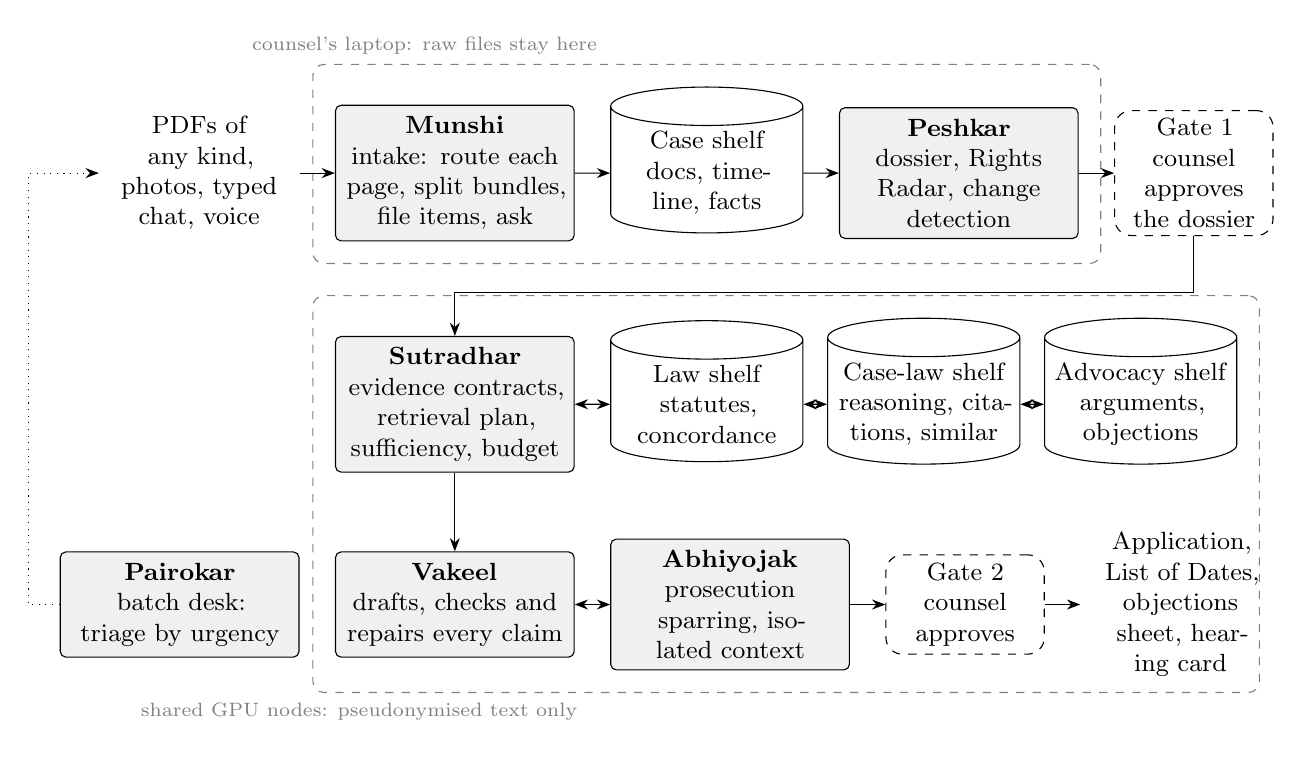
\begin{tikzpicture}[
  font=\small, >=Stealth,
  ag/.style={draw, rounded corners=2pt, fill=gray!12, align=center, inner sep=4pt, minimum height=0.8cm, text width=2.75cm},
  st/.style={draw, cylinder, shape border rotate=90, aspect=0.2, align=center, inner sep=2pt, minimum height=1.0cm, text width=2.3cm, fill=white},
  gt/.style={draw, dashed, rounded corners=6pt, align=center, inner sep=3pt, text width=1.8cm, fill=white},
  io/.style={align=center, text width=2.3cm}]
% laptop column
\node[io] (in) {PDFs of any kind, photos, typed chat, voice};
\node[ag, right=0.45cm of in] (mu) {\textbf{Munshi}\\ intake: route each page, split bundles, file items, ask};
\node[st, right=0.45cm of mu] (case) {Case shelf\\ docs, timeline, facts};
\node[ag, right=0.45cm of case] (pe) {\textbf{Peshkar}\\ dossier, Rights Radar, change detection};
\node[gt, right=0.45cm of pe] (g1) {Gate 1\\ counsel approves the dossier};
% server row
\node[ag, below=1.2cm of mu] (su) {\textbf{Sutradhar}\\ evidence contracts, retrieval plan, sufficiency, budget};
\node[st, right=0.45cm of su] (law) {Law shelf\\ statutes, concordance};
\node[st, right=0.3cm of law] (cl) {Case-law shelf\\ reasoning, citations, similar};
\node[st, right=0.3cm of cl] (adv) {Advocacy shelf\\ arguments, objections};
\node[ag, below=1.0cm of su] (va) {\textbf{Vakeel}\\ drafts, checks and repairs every claim};
\node[ag, right=0.45cm of va] (ab) {\textbf{Abhiyojak}\\ prosecution sparring, isolated context};
\node[gt, right=0.45cm of ab] (g2) {Gate 2\\ counsel approves};
\node[io, right=0.45cm of g2] (out) {Application, List of Dates, objections sheet, hearing card};
\node[ag, left=0.45cm of va] (pa) {\textbf{Pairokar}\\ batch desk: triage by urgency};
\draw[->] (in) -- (mu); \draw[->] (mu) -- (case); \draw[->] (case) -- (pe); \draw[->] (pe) -- (g1);
\draw[->] (g1.south) |- ($(su.north)+(0,0.55)$) -- (su.north);
\draw[<->] (su) -- (law); \draw[<->] (law) -- (cl); \draw[<->] (cl) -- (adv);
\draw[->] (su) -- (va); \draw[<->] (va) -- (ab); \draw[->] (ab) -- (g2); \draw[->] (g2) -- (out);
\draw[dotted,->] (pa.west) -- ++(-0.4,0) |- (in.west);
\begin{scope}[on background layer]
 \node[draw=gray, dashed, rounded corners, fit=(mu)(case)(pe), inner sep=0.28cm, label={[font=\scriptsize,gray]above left:counsel's laptop: raw files stay here}] {};
 \node[draw=gray, dashed, rounded corners, fit=(su)(law)(cl)(adv)(va)(ab), inner sep=0.28cm, label={[font=\scriptsize,gray]below left:shared GPU nodes: pseudonymised text only}] {};
\end{scope}
\end{tikzpicture}
\caption{Architecture. Munshi, Peshkar and the case shelf run on counsel's machine; Sutradhar, Vakeel and Abhiyojak see pseudonymised text only. Both gates are enforced in code.}
\label{fig:arch}
\end{figure*}

\paragraph{Agents.} \textbf{Munshi} (intake) decides the parse route of each page, when to escalate, document boundaries and types, where each item is filed, and what is missing. \textbf{Peshkar} builds the dossier with a source quote for every field, a List of Dates, and the Rights Radar (deterministic checks on custody periods and statutory rights, each with a verification status). \textbf{Sutradhar} orchestrates retrieval. \textbf{Vakeel} drafts the grounds and checks and repairs every claim. \textbf{Abhiyojak} plays the prosecution with its own prompt and an allow-listed context. \textbf{Pairokar} orders a batch by urgency and decides per case between a full brief, a flag for counsel, or a request for documents. Every action is appended to an event log; dossier, timeline, brief and sparring record are views of it, which gives an audit trail and the dependency data for truth maintenance.

\paragraph{Ingestion ladder.} Munshi handles ten input kinds (born-digital, scanned, degraded, phone photo, Hindi or mixed script, legacy Hindi fonts, handwriting, bundles, locked files, non-PDF). A page climbs only as far as needed: text layer; layout parser; clean-up and OCR; a vision model asked only to transcribe; a request to counsel for a clearer copy. Per-page quality signals (text coverage, OCR confidence, dictionary-word share, script, legacy-font patterns) decide each step and are logged. A gap-driven re-read returns to a page when a checklist field is still missing. The ladder is evaluated as a router against the cheapest route that clears the quality bar.

\paragraph{Ten stores on four shelves.} A brief needs exact text, a section-mapping graph, court reasoning, citation history, what each side usually argues, and the client's own record; each has a different right way to search. The \emph{law} shelf holds statutes (exact lookup, BM25) and the IPC--BNS and CrPC--BNSS concordance (typed graph). The \emph{case-law} shelf holds reasoning paragraphs (BM25 plus BGE-M3, metadata pre-filter), the citation graph with treatment and court level, and whole-order fact vectors. The \emph{advocacy} shelf holds defence-argument and prosecution-objection paragraphs by factor, used for coverage and phrasing, never cited as authority. The private \emph{case} shelf holds the client's documents in structure-aware chunks, a dated timeline and the dossier. The October 2026 build has 161,708 reasoning paragraphs, 70,880 arguments, 55,161 objections, 114,692 similar-fact orders and 5,842 citation edges (37.3\% of citations resolved to a document). Test-window orders and same-FIR orders are excluded from every store.

\paragraph{Evidence contracts and the orchestrator.} Each of twelve bail factors has a contract: slots (for example co-accused order, role comparison, authority, good-law check, likely objection), a need for each (required, a count, or optional), the stores that may hold it, and a budget in store calls and tokens. Sutradhar decides whether the factor applies, the order of calls, the query and filters, whether a result is good enough, when to relax a filter or follow a citation, and when to stop; slots left unfilled become open issues, never silent omissions. A learned store prior, trained from train orders, may order calls within a contract (S6) or replace the contracts (B5).

\paragraph{Checking and truth maintenance.} Vakeel checks every claim with an NLI model and rules (statute lookup, section mapping, good-law check), and repairs or flags it; nothing is dropped silently. Each claim records the dossier fields (by hash), timeline events, rights entries and authorities it depends on. When counsel approves a change, claims with a changed dependency, and claims citing them, become stale; only the reopened factors are re-planned, and unchanged claims stay byte-identical (tested).

\paragraph{Gates and privacy.} Gate 1 (dossier) and Gate 2 (brief) pass only on counsel's approval, and export is impossible before Gate 2, in code and in tests. Raw client files stay on the user's machine. External model services are off by default, gated by a mode (\texttt{off}, \texttt{public}, \texttt{pseudonymised}, \texttt{consented}) and per-case consent, and every external payload passes the pseudonymisation boundary. Defences against instructions planted in documents (a typed hand-off from a tool-less extractor, spotlighting, a guard) are built as arms of the safety test set T7; \todo{owner Shravani: state which defences are on by default}.

\paragraph{Models.} Munshi and Peshkar are specified for a 4B model with OCR and a vision model on an 8 GB laptop GPU; Sutradhar, Vakeel and Abhiyojak for a 14B model on shared GPU nodes. The runs reported here use a hosted model (OpenAI) behind the privacy boundary; a Sarvam-105B arm is planned. Helper models: BGE-M3, a DeBERTa NLI model, MiniCheck.

\section{Evaluation Design}
\label{sec:eval}

The evaluation follows the course material on evaluation (L12) and on RAG evaluation (L14): state the evaluated object, decide the claims, thresholds and tests before looking at results, seal a slice, report intervals, and audit the metrics themselves. No score comes from an LLM judge, and no label is made by hand.

\paragraph{Test sets.} Nine sets built from court text, official tables or construction. \textbf{T1}: 200 High Court test-window orders (at least 60 BNS-era), facts part as input, plus 50 dev orders. \textbf{T2}: 600 messy bundles with known text, boundaries and fields, and 200 native Hindi High Court orders. \textbf{T3}: 240 change-set updates. \textbf{T4}: 627 rights scenarios from the written rule table (a conformance check of the Radar against its specification, not a legal one). \textbf{T5}: 300 batch cases with planted deadlines. \textbf{T6}: 150 chat questions. \textbf{T7}: 60 safety scenarios. \textbf{T8}: 300 utterances (Kathbath Hindi, dictated facts). \textbf{T9}: 2,095 citation strings.

\paragraph{Gold labels without annotators.} Seven kinds of gold label are derived from the order text. G1 is the set of the 12 bail factors the defence argued; G2 the precedents the court cited that resolve to a document in the index; G3 dossier fields and dated events (sections, dates, charge-sheet status, co-accused bail, stage); G4 the objections the prosecution raised; G5 the factors the court discussed; G6 condition types of the operative order; G7 the rights computations the court states itself (custody against the 60 and 90 day limits, s.436A and s.479). For G1 and G3 (and, with weaker coverage, G4 to G6) two labelers work independently: the keyword and date rules, and a hosted model (OpenAI \texttt{gpt-6-luna}) that is not shown the rule output. This labeler is the same model as the system in the dev runs, so the agreed gold is not independent of the system; the rule-only gold is therefore reported beside it as a co-primary column. A label enters gold only if both agree, and the labeler must quote a verbatim span, which is rejected unless it is found in the order (a date label needs a written date in the span that normalises to the claimed date). The agreed gold is primary; the rule-only gold is a declared secondary, and every headline metric is also recomputed on it (label-source sensitivity). Table~\ref{tab:kappa} gives agreement on 250 orders (200 test plus 50 dev); a second labeler (Sarvam-105B) on a random 80 orders gives $\kappa = 0.78$ for G1 against the first labeler. G2 is rule-extracted and merged from the Supreme Court metadata index; dev has no resolved citation (0 of 50), so recall of court-cited precedents is undefined on dev and measurable on the test slice only (14 of 200 orders).

\begin{table}[!t]
\centering\small
\begin{adjustbox}{max width=\textwidth}
\begin{tabular}{lrrr}
\toprule
Gold & $\kappa$ & 95\% CI & orders with label \\
\midrule
G1 factors & 0.60 & [0.55, 0.64] & 169 of 250 \\
G3 fields & 0.84 & [0.82, 0.86] & 249 of 250 \\
\bottomrule
\end{tabular}
\end{adjustbox}
\caption{Agreement of the rules and the model labeler (pooled $\kappa$, bootstrap over orders). G1 is weakest on gravity ($\kappa$ 0.27) and weak prima facie case (0.25); G3 on previous bail (0.26). G7 has a label for 1 of 250 orders, so claims on rights rest on T4.}
\label{tab:kappa}
\end{table}

\paragraph{Leakage control.} Train orders (before 2024) feed the stores. Test and same-FIR orders are excluded from every store, and an 8-word-overlap check compares each test order's facts with every store paragraph. Dev is open to everyone. Of the 200 test orders, 120 are open for analysis after the freeze and 80 form a blind slice, drawn with a seed before the freeze (at least 25 BNS-era) and hashed into the pre-registration. It is scored once, and a claim is supported only if it also holds there.

\paragraph{Pre-registration.} \texttt{docs/preregistration.md} fixes, before the first test-set run, the claims with dev-fixed thresholds, the switch set, prompt hash and code tag, metric definitions, seeds, tests and Holm families, reporting rules, and what may change after the freeze. It is a template at this date; the freeze tags do not exist yet.

\paragraph{Baselines.} All RQ1 systems use the same model, the same 12-factor checklist and the same pseudonymised facts, so no gain comes from a larger model or cleaner input. \textbf{B0}: single pass, facts and checklist to brief in one call. \textbf{B0L}: B0 on a larger prompted model (Sarvam-105B in the plan; \texttt{gemini-3.6-flash} in the runs reported here, because Sarvam is locked). \textbf{B1}: one store, top-10 by facts, one drafting call. \textbf{B2}: whole-order embeddings (BGE-M3, 8K), top-3 orders in full. \textbf{B3}: B1 with naive chunking (fixed 512, overlap, recursive, semantic, page). \textbf{B4}: every store queried and fused by reciprocal rank, no orchestrator. \textbf{B5}: a learned store router without contracts. \textbf{B6}: an expert rule checklist with no model. These map to the four baseline types of the course: a prompted large model (B0L), the base small model (optional B0S), retrieval without an agent (B1 to B3), and the simplest expert rule (B6). B6 does not reuse the keyword tagger that builds gold, and its factor recall is not used as evidence, since arguing all twelve factors has recall 1.0 by construction; that rule's F1 is printed in every table as a floor.

\paragraph{Ablations and variants.} Every change is a field of one typed \texttt{Switches} object, so an ablation is a flag and not a code fork. The core ablations remove one part at a time: the dossier (A1), check and repair (A2), tools (A3), the factor filter (A4), the fine-tuned extractor (A5), contracts (A6, A7), sparring (A8), and one store (A10). On top of these are 18 variants (S1 to S18) and four ingestion arms (P5 to P8), each adapted from a paper checked on its official page (Appendix~\ref{app:arms}). Every variant is opt-in, leaves default behaviour byte-identical, and has a switch, an effect test and a row in the literature-to-code map; none reproduces its paper. An offline audit runs 61 of 61 ids end to end, and 42 effect tests check that switches change behaviour.

\paragraph{Metrics.} Headline: factor recall, lenient and strict precision, and F1 against the argue-all floor (M1 to M3); the unsupported-fact rate by MiniCheck (RoBERTa-Large; the scorer refuses to use the system's own DeBERTa checker) plus a verbatim-span check (M6), with a faithful/corroborated table that separates ``unsupported'' from ``wrong''; fabricated citations (M9); recall@$k$, MRR and nDCG of court-cited precedents with coverage columns (M10, M11; L14, ``gold document in the top $k$''); slot fill (M12); good-law violations with a known-treatment share (M15); ALCE-style citation precision and recall and removal faithfulness (M16, M17); stopping quality (M18); the coverage-risk curve (M33); and tokens, calls, latency and USD with the cost-quality frontier. Ingestion uses character error rate, boundary F1 and field accuracy. The full list is in Appendix~\ref{app:metrics}.

\paragraph{Statistics.} The unit is the case; runs are averaged within a case. Paired comparisons use a 95\% bootstrap interval of the mean difference (10,000 resamples of cases) with Wilcoxon signed-rank as confirmation; binary outcomes use McNemar's test (exact below 25 discordant pairs); pooled item-level data resample cases, not items; non-inferiority uses a margin fixed on dev. Holm correction applies inside each pre-registered family (Full against B0, B0L, B1, B2, B3, B4 on recall is one family of six) for per-baseline statements; claim C1 (Full beats every baseline) is an intersection-union test, supported only if every comparison is significant at $\alpha$, and incomplete while a baseline has not run. Slices under 20 cases are marked too few, best-of-$N$ is forbidden, and safety counts are bounded by the rule of three, not tested.

\paragraph{Auditing the metrics.} Five degenerate agents (empty brief, copy the facts, copy the checklist, argue all twelve factors, random citations) must score near the floor the plan predicts, so no metric rewards doing nothing. The scoring loader refuses to mix runs from different commits.

\section{Preliminary Results}
\label{sec:results}

\paragraph{What this section is.} A template. Every number in it comes from a table written by the scoring pipeline (\texttt{python -m vakeel\_sahayak.eval.scoring score} then \texttt{report}), which writes LaTeX fragments to \texttt{docs/results/dev-sweep/tables/}. The document includes them when they exist and shows a placeholder when they do not. No number is typed in the text. Where a sentence needs one, a \todo{} marker names the table that holds it.

\paragraph{What ran.} The baselines \texttt{full} (two runs), \texttt{b0}, \texttt{b1}, \texttt{b4} and \texttt{b6} were rerun on all 50 dev cases from a clean worktree of the tag \texttt{dev-sweep-v1} (commit \texttt{efd0ce4}); every manifest carries the code stamp, and the scorer refuses to mix commits. The backend is OpenAI \texttt{gpt-6-luna} behind the pseudonymisation boundary, with the real DeBERTa NLI as claim checker. A hosted stand-in for B0L duplicated B0 (same model and prompt) and was dropped; the real B0L is a Sarvam-105B single pass and has not run. Earlier runs carry a dirty-tree stamp and are not scored. The variants and studies of Appendix~\ref{app:arms} are planned; \todo{owner Vishak: which phases have run by the submission date}. Scoring is on the dev slice, agreed gold primary, rule-only gold secondary.

\paragraph{Main comparison.} \resref{table1_main} compares Full with the baselines on factor recall, lenient precision, F1, unsupported-fact rate, recall@10 of court-cited precedents (undefined on dev, see Section~\ref{sec:eval}), objection recall, pass$^k$ and tokens. \todo{one sentence from table1\_main: Full vs.\ B0 to B4 on recall and unsupported-fact rate, with the 95\% interval and n; state whether the intervals overlap}. \todo{one sentence from table\_paired and table\_holm: which of the six recall comparisons survive Holm}.

\resulttable{table1_main}{w}

\paragraph{What each baseline shows.} B0 (single pass) isolates the effect of having no retrieval and no agents: \todo{from table1\_main}. B1 and B3 (one store, with or without naive chunking) isolate the effect of several typed stores against one: \todo{from table1\_main}. B2 (whole-order embeddings) isolates retrieval granularity: \todo{b2 has not run; owner Vishak}. B4 (every store, fused) isolates an agent choosing against querying everything, and its token cost against Full: \todo{table1\_main and table9\_cost}. B6 (expert rule list) gives the no-model floor and is scored on precision, unsupported-fact rate and the Rights checks only: \todo{from table1\_main and table\_rights}. B5 and B0L: \todo{not run}.


\paragraph{Variants sweep.} Variants S1 to S18 and the ablations are compared with Full on the same backend and the same cases, so each comparison is paired. The offline studies (scheduling S14b and S14c, chunk strategies S16 and S16b, retrieval S4 and S5, removal M17) run at zero model cost. \todo{variants table and a sentence on which variants move M1 or M6 beyond their interval; table not yet generated, owner Satvik for the Sarvam block, Vishak for the OpenAI and offline phases}. S6 and B5 have no effect until a store prior is trained; the train-order labelling this needs is not done.

\paragraph{Label-source sensitivity.} The same outputs are scored against the agreed gold and the rule-only gold. \resref{table_sweep_metrics} shows both and the difference; \todo{one sentence: does the ordering of systems change with the label source? from table\_sweep\_metrics and table\_sweep\_robustness}.


\paragraph{Cost.} \resref{table9_cost} gives tokens, store calls, latency and USD per case. \todo{one sentence from table9\_cost: Full vs.\ B4 token ratio (plan expects about 1.0 to 1.6) and Full vs.\ B0}.


\section{Limitations and Risks}

\begin{itemize}\setlength\itemsep{0pt}
\item \textbf{Small $n$, dev only.} All runs use the 50 dev orders (25 for some arms); intervals will be wide and the blind slice is unopened.
\item \textbf{Stand-in models.} Offline arms use a template LLM and, unless MiniCheck or the DeBERTa NLI is installed, an offline NLI; such numbers carry that label in the tables. The 4B and 14B models of the design have not been run on the GPU nodes for this report.
\item \textbf{Thin facts in T1.} The facts part is often only a caption. A single pass then answers ``no facts supplied'', while Full draws grounds from retrieved authorities not tied to the client's facts, so Full can win on recall through retrieved boilerplate.
\item \textbf{Gold is not human.} Rules plus one non-Qwen labeler that must agree; $\kappa$ is 0.60 for G1, and the agreed G1 gold leaves 81 of 250 orders without a factor. Only 37.3\% of citations resolve, and no dev order has a resolved court citation. HLDC was unavailable, so the Hindi set is native High Court orders from one court and two years.
\item \textbf{Rights Radar.} All seven rules are marked unverified until the owner re-checks them against the bare acts and cited judgments.
\item \textbf{No authentication.} The gates are enforced in code, but there are no user accounts, so ``approval only from counsel'' is a property of the code path, not of an identity check.
\item \textbf{Budgets.} OpenAI is capped by a ledger (ceiling 4.90 USD), the owner's Sarvam key at INR 30; a larger Sarvam block runs on a teammate's key. The full plan (about 4,500 Full case-runs) does not fit, so sample sizes are cut, not features.
\item \textbf{Known weaknesses.} Grounds are sometimes weak in substance (about ten open issues per case; sparring objections mostly unanswered); the pseudonymiser still refuses one order of 250.
\end{itemize}

\section{Threats to Validity}
\label{sec:threats}

\paragraph{Internal.} Small $n$ and a single run for most arms limit what can be resolved; an effect smaller than the interval is reported as not resolved. Thresholds fixed on 50 orders may be mis-set, so margins are rounded to whole points; the pass bar and NLI threshold are provisional until the freeze.

\paragraph{Construct.} Gold from rules plus a non-Qwen LLM labeler, not humans, risks circularity: the system reads the facts part of an order while gold is read from other parts of the same order, and the tagger that builds paragraph metadata is of the same family as the rule labeler. Controls are an 8-word-overlap check, agreed labels, label-source sensitivity, and B6 not reusing the tagger. Because T1 facts are often only a caption, retrieved boilerplate can inflate recall; the answerable-factor rule and the faithful/corroborated table are guards, not a cure. Factor recall against G1 measures what the defence argued, not what a good lawyer should argue; lenient precision against G1 $\cup$ G5 corrects this in part. The NLI checker is a stand-in or a model validated on other domains, so subtle legal entailment errors may pass.

\paragraph{External.} One legal domain (bail), one source of orders, one court for the Hindi native set, and constructed data for T2 to T5, T7 and T8 limit transfer. Only 5.9\% of orders split cleanly, so results hold for orders that split cleanly. Qwen3 and the hosted labeler may have seen public orders; the release date bounds the cutoff but does not measure it. There is no user study, and no claim about lawyer time or outcomes.

\section{Status and Plan}
\label{sec:status}

\paragraph{Done.} The six agents and the event log; the ten stores; the ingestion ladder; contracts and Sutradhar; Vakeel's check and repair; Abhiyojak; truth maintenance with the byte-identity test; Pairokar; the Rights Radar (rules unverified); both gates and the privacy boundary; the web interface and API routes. For evaluation: test sets T1 to T9, gold G1 to G7 (Table~\ref{tab:kappa}), baselines B0 to B6, every S/A/P variant as a switch (61 of 61 pass an offline end-to-end audit; 42 effect tests), the scoring pipeline (bootstrap, Wilcoxon, McNemar, cluster bootstrap, Holm), the label-source sweep, the offline studies, the code stamp in every manifest, and spend ledgers for both hosted providers. The suite has 4,514 passing unit tests with integration and system tests green; \todo{owner Vishak: final counts and the three open test-versus-design conflicts on the report date}.

\begin{table}[t]
\centering\small
\begin{tabular}{@{}p{3.6cm}p{1.5cm}p{1.5cm}@{}}
\toprule
Item & State & Owner \\
\midrule
Score dev reruns at tag \texttt{dev-sweep-v1} & to do & Vishak \\
OpenAI ablation arms (phase 2) & not run & Vishak \\
Sarvam block, B0L on Sarvam-105B & not run & Satvik \\
Ada phase (local 4B) & not run & Vishak \\
Trained store prior (S6, B5) & not done & Vishak \\
Rights rule verification & pending & Harshita \\
Privacy root-cause fix & in review & Shravani \\
Freeze tags, pre-registration & template & all \\
Blind-slice run, once & after freeze & all \\
\bottomrule
\end{tabular}
\caption{Work left. Owners follow the split of the project file.}
\label{tab:status}
\end{table}

\paragraph{Next, to the freeze.} (1) Score the existing dev reruns, which needs no paid call. (2) Run the zero-cost offline phase, then, when the key arrangement allows it, the OpenAI ablations and the Sarvam block. (3) Fix thresholds on dev, fill the pre-registration, create \texttt{prereg-v1} and \texttt{eval-freeze-v1}, and run from a clean worktree of the freeze tag. (4) Open the blind slice once. (5) Case studies from the failure taxonomy. \todo{owner: dates for each step and the submission date}.

\paragraph{Risks.} Budget: the plan needs more calls than the caps buy, so sample sizes shrink first and features never (cut order is in the plan). Compute: shared GPU nodes and a laptop with about 97\% disk use. Gated resources: HLDC and an Indic translation model are not yet available. Gold quality: low agreement on two factors may force a merge of confusable factors. A null result on any claim is reported as such.

\section*{Ethics and Privacy Statement}

Client files stay on the user's machine. Text leaves it only through the pseudonymisation boundary, and only when the external-model mode and per-case consent allow it; external services are off by default. On 250 T1 orders the party-name proxy check leaked 80 orders' names before a fix to caption-name learning and 5 after. We have not claimed zero leakage. Keys live in environment variables, never in the repository, and spending is capped in code. The public corpus is court text already in the public domain; orders with the same FIR as a test order are excluded from the stores. The system makes no outcome predictions, shows no grant rates, and gives no advice to accused persons or the public; the landing page points them to free legal aid (NALSA helpline 15100). Export needs counsel's approval at Gate 2. Constructed test cases use synthetic names. No manual annotation was used.


\bibliography{references}

\appendix
\section{Reproducibility}
\label{app:repro}

\paragraph{Code and data.} The repository is the code of record; the pinned tag for the dev reruns is \texttt{dev-sweep-v1} (commit \texttt{efd0ce4}). Data (\texttt{interim}, stores, test sets, gold, and the raw sources: Open India Law shards, IPC2BNS-Verify, Kathbath) is not in the repository. It is a private dataset in the Hugging Face organisation \texttt{Vakeel-Sahayak}, \texttt{vakeel-sahayak-data}; access is granted by the owner. Helper models (BGE-M3, DeBERTa NLI, MiniCheck, Whisper small) are fetched by \texttt{make models}.

{\footnotesize\begin{verbatim}
make setup
make data
make models
make smoke        # case-0007, offline
make eval-smoke
python -m vakeel_sahayak.eval.runners.driver \
  plan --sweep
python -m vakeel_sahayak.eval.scoring score \
  --runs data/eval/dev_runs --slice dev \
  --gold-source both --out data/eval/dev_scores
python -m vakeel_sahayak.eval.scoring report \
  --scores data/eval/dev_scores
\end{verbatim}}

\paragraph{Manifests.} Each run writes a manifest with the system id and variant, prompt hash, config hash, model names and modes, test-set and gold hashes, shard count, and the code stamp (\texttt{git\_sha}, \texttt{git\_dirty}, \texttt{code\_tree\_hash}). The scoring loader refuses runs from different commits unless told otherwise, and a dirty stamp is not admissible for frozen runs. The hosted-model settings are \texttt{VS\_MODELS=auto}, \texttt{VS\_LLM\_BACKEND=openai}, \texttt{VS\_EXTERNAL=pseudonymised}, with keys read from an untracked \texttt{.env}; offline stand-ins are the default and need neither a GPU nor a key. Agreed-gold hashes: \todo{owner Vishak: paste cases, dev and gold sha256 from the manifest at the report date}.

\section{Arms}
\label{app:arms}

\begin{table*}[t]
\centering\small\setlength\tabcolsep{3pt}
\begin{tabular}{@{}lp{5.2cm}p{3.5cm}l@{}}
\toprule
Id & Idea (source) & Switch & Run so far \\
\midrule
B0, B1, B4, B6, Full & baselines (Section~\ref{sec:eval}) & driver system id & dev, pinned tag, not scored \\
B0L, B2, B3, B5, B0S & baselines & driver system id & not run \\
S1 & self-critique retrieval \citep{asai2024selfrag,yan2024crag} & \texttt{retrieval\_policy} & planned \\
S2 & adaptive depth \citep{jeong2024adaptive} & \texttt{retrieval\_policy} & planned \\
S3, S3b & sufficiency stopping \citep{joren2025sufficient} & \texttt{stopping} & planned \\
S4 & score-skew weak signal & \texttt{weak\_signal} & offline study \\
S5 & citation-graph expansion \citep{gutierrez2025hipporag2} & \texttt{graph\_expansion} & offline study \\
S6 & learned store prior \citep{zhang2026agentrouter} & \texttt{store\_prior} & needs trained prior \\
S7 & hierarchy re-reading for Munshi & \texttt{munshi\_gap\_policy} & planned (T2) \\
S8 & self-critique repair \citep{gou2024critic,huang2024selfcorrect} & \texttt{repair\_mode} & planned \\
S9, S10 & sampling critic; no isolation \citep{choi2025debate,wynn2025talk} & \texttt{critic\_mode}, \texttt{abhiyojak\_isolation} & planned \\
S11 & three-role review, debate, vote \citep{kumar2025courtevel} & \texttt{critic\_mode}, \texttt{draft\_mode} & planned \\
S12 & topology: sequential, single agent \citep{cemri2025mast} & \texttt{topology} & planned \\
S13 & searched workflow (grid on dev) & none (grid over switches) & offline smoke \\
S14, S14b--d & plan cache, scheduling, prefix signal \citep{zheng2024sglang} & \texttt{plan\_cache}, \texttt{urgency\_policy} & offline study \\
S15, S15b & output format \citep{tam2024speak} & \texttt{output\_format} & planned \\
S16, S16b & proposition units, late chunking \citep{chen2024densex} & \texttt{chunking} & offline study \\
S17 & injection defences \citep{beurerkellner2025patterns} & defence flags & planned (T7) \\
S18 & authority stance \citep{wachsmuth2018} & stance switch & planned \\
P5--P8 & ingestion arms, image-only \citep{yu2025visrag,faysse2025colpali} & \texttt{munshi\_*} & planned (T2) \\
A1--A10 & remove one part (dossier, repair, tools, filter, extractor, router, planner, sparring, a store) & \texttt{Switches} flags & planned \\
\bottomrule
\end{tabular}
\caption{Arms and their state. ``Planned'' means the arm is implemented and offline-smoked, with a phase in the sweep plan, and has not produced scored results. Switch names follow \texttt{orchestration/switches.py}; \todo{owner Vishak: check the S18 and S3b switch names}.}
\end{table*}

\section{Metrics}
\label{app:metrics}

\begin{table*}[t]
\centering\small
\begin{tabular}{@{}llp{6.2cm}l@{}}
\toprule
Id & Metric & Definition and check & Set \\
\midrule
M1--M3 & factor recall, precision, F1 & set comparison with G1 (and G5 for lenient precision) on answerable factors; argue-all F1 as floor & T1 \\
M4 & G5, G4, G6 recall & as M1 for court-discussed factors, objections, conditions & T1 \\
M5 & label-source sensitivity & M1 to M4 on rules-only, labeler, agreed; $\kappa$ per factor & T1 \\
M6 & unsupported-fact rate & share of factual sentences MiniCheck or the NLI finds unsupported & T1 \\
M7 & factual error & wrong section, date, statute text, custody count against tools & T1 \\
M9 & fabricated citation & id not in index, or span not found verbatim & T1 \\
M10, M11 & recall@$k$, MRR, nDCG@10 & court-cited precedents, with coverage columns & T1 \\
M12 & slot-fill rate & required slots filled; missing slots are open issues & T1 \\
M13, M15 & authority quality, good-law violations & metadata and graph lookup; known-treatment share & T1 \\
M16, M17 & citation precision, recall; removal & ALCE-style; claims unchanged when the paragraph is removed & T1 \\
M18 & stopping quality & over-search and stopped-too-early & T1 \\
M19 & weak-evidence AUROC & score skew predicts a top-10 gold hit & T1 \\
M33 & coverage-risk & abstention curve & T1 \\
Ingestion & CER, boundary F1, type and field accuracy & against construction truth; escalation, GPU seconds & T2 \\
Rights & accuracy, false-ELIGIBLE & designed answers by construction; Wilson interval & T4 \\
Safety & attack success, unapproved exports & bounded by the rule of three & T7 \\
Cost & tokens, calls, latency, USD & from manifests and ledgers; cost-quality frontier & all \\
\bottomrule
\end{tabular}
\caption{Metrics. Definitions are in the evaluation plan; none is an LLM-judge score.}
\end{table*}

\section{Glossary of Names Used in This Report}
\label{sec:glossary}

\begin{description}\itemsep0pt
\item[Full] The complete system: all six agents, the ten stores, retrieval, verification and prosecution sparring.
\item[B0 to B6] Baselines, simpler systems that Full must beat. B0: one model call with no retrieval. B1: retrieval from one store. B2: retrieval over whole-order embeddings. B3: retrieval over naively chunked text. B4: every store searched and fused, with no agent planning. B5: a learned router alone, with no contracts. B6: rules only, no model. B0L: B0 on a larger model.
\item[A1 to A10] Ablations: Full with one part switched off, to show whether the part earns its place.
\item[S1 to S18] Variants taken from the literature (Section~\ref{sec:literature}). Each swaps one idea from a paper into the system as an opt-in switch. P5 to P8 are the same for intake.
\item[Dev set] The 50 development orders (T1 dev). All numbers in this report come from it. The blind slice has not been opened.
\item[Code tag] A named snapshot of the code. \texttt{dev-sweep-v1} (27 October) is the code of the first 50-case baseline runs; it is superseded and reported only as such. \texttt{dev-sweep-v3} (29 October) is the current code; every other model run reported here comes from it. A result is comparable only with results from the same tag, and the scorer refuses to mix tags.
\item[Block] A batch of runs on one model and one set of cases: the OpenAI block (\texttt{gpt-6-luna}), Gemini block A (\texttt{gemini-3.5-flash-lite}) and Gemini block B (\texttt{gemini-3.1-flash-lite}). Arms are compared only with the Full of the same block (Table~\ref{tab:models}).
\item[Agents] Munshi (intake), Peshkar (dossier and Rights Radar), Sutradhar (orchestrator), Vakeel (drafter), Abhiyojak (prosecution sparring), Pairokar (batch desk).
\item[Gates] Gate 1 (dossier) and Gate 2 (brief): approvals that only counsel can give; export is impossible before Gate 2.
\item[Metrics] M1 to M35, listed in the metrics table of this appendix: M1 factor recall, M6 unsupported-fact rate, M10 recall of cited precedents, and so on.
\end{description}

\section{Further Generated Tables}

\resulttable{table_paired}{w}
\resulttable{table_holm}{w}
\resulttable{table_sweep_metrics}{w}
\resulttable{table9_cost}{w}
\resulttable{table_label_coverage}{n}
\resulttable{table_label_sensitivity}{w}
\resulttable{table_label_kappa}{n}
\resulttable{table_citations}{w}
\resulttable{table_abstention}{w}
\resulttable{table_rights}{n}
\resulttable{table_sweep_robustness}{w}


\end{document}
